\documentclass[aspectratio=169,11pt]{beamer}
\usepackage{teaching_slides}

\title[L13b - Duration Models]{ Econometrics I}
\subtitle{Lecture 13b: Duration Models}
\author{Chris Conlon \\NYU Stern}
\date{Fall 2026}

% New deck (Fall 2026). Readings: Wooldridge Ch. 22; Kiefer (1988, JEL) "Economic
% Duration Data and Hazard Functions"; Cameron & Trivedi Ch. 17 for more.
% Figures/tables simulated with known ground truth: ldv_sims.R (Part B).
% Workbook: inclass_session13.Rmd

\begin{document}
\maketitle

\begin{frame}{Durations}
\begin{itemize}
	\item The outcome is a \alert{length of time until something happens}: months until a subscriber
	cancels, days until a loan defaults, quarters until a firm exits, weeks until a job seeker is hired,
	years until a patent is cited.
	\medskip
	\item Two features make this its own subject:
	\begin{enumerate}
		\item \alert{Censoring.} When the data end, many spells are still running. You know the
		duration is \emph{at least} $c_i$. Throwing those out, or treating them as completed, is wrong
		in opposite directions.
		\item \alert{The question is about timing.} ``Does a price increase raise churn?'' means
		``does it raise the \emph{rate} at which subscribers leave, given they are still here?'' That
		object is the hazard, and it is what business users of these models actually want.
	\end{enumerate}
	\medskip
	\item Readings: Wooldridge Ch.~22; Kiefer (1988, \emph{JEL}).
\end{itemize}
\end{frame}


\begin{frame}{Survival and hazard functions}
Let $T \ge 0$ be the duration, with CDF $F(t)$ and density $f(t)$.
\begin{align*}
	S(t) &= \Pr(T > t) = 1 - F(t) && \text{\alert{survival function}: share still ``alive'' at } t \\[4pt]
	h(t) &= \lim_{\Delta \to 0} \frac{\Pr(t \le T < t + \Delta \mid T \ge t)}{\Delta} = \frac{f(t)}{S(t)}
	&& \text{\alert{hazard}: exit rate at } t \text{, given survival to } t
\end{align*}
\begin{itemize}
	\item Since $f = -S'$, $h(t) = -\frac{d}{dt}\ln S(t)$, so $S(t) = \exp\big(-\int_0^t h(u)\,du\big) \equiv e^{-\Lambda(t)}$.
	The hazard determines everything: model it, and $S$, $f$, and $\E[T]$ follow.
	\item The hazard is what the decision-maker faces \emph{now}: ``of the subscribers still with us at
	month $6$, what fraction leave in month $7$?''
	\item Discrete time: $h_t = \Pr(T = t \mid T \ge t)$, $S(t) = \prod_{s \le t}(1 - h_s)$: a sequence
	of binary choices, which is why a logit with time dummies is a duration model.
\end{itemize}
\end{frame}


\begin{frame}{Duration dependence: what shape is the hazard?}
\begin{center}
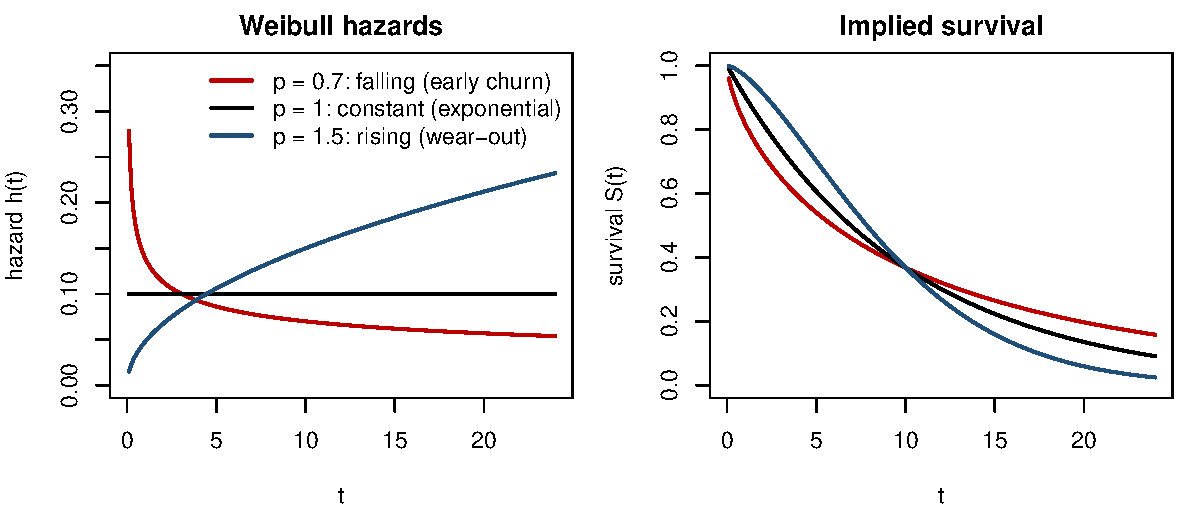
\includegraphics[width=.66\textwidth]{fig_dur_hazards.pdf}
\end{center}
\vspace{-.2cm}
\begin{itemize}
	\item \alert{Constant} hazard (exponential): memoryless; the expected remaining life never changes.
	\item \alert{Falling} hazard: churn concentrated early (trial users), default risk highest in the first
	year of a loan.
	\item \alert{Rising} hazard: wear-out; contract renewal dates; a job search whose reservation wage drifts down.
\end{itemize}
\end{frame}


\begin{frame}{Running example: subscription churn}
\begin{itemize}
	\item $3{,}000$ subscribers. Covariates: whether they experienced a \alert{price increase} (half did)
	and their standardized \alert{usage}.
	\medskip
	\item True hazard, Weibull with proportional covariate effects:
	\begin{align*}
		h(t \mid x) = \underbrace{p\,t^{\,p-1}}_{\text{baseline}} \cdot \exp(\alert{0.5}\cdot\text{price} \alert{\ -0.4}\cdot\text{usage}), \qquad p = 0.7 .
	\end{align*}
	A price increase multiplies the exit rate by $e^{0.5} \approx 1.65$ at every $t$. Falling baseline:
	early churn.
	\medskip
	\item We observe subscribers for $24$ months; some also drop out of the panel early for unrelated
	reasons. About a quarter of spells are \alert{right-censored}: we know they lasted at least $c_i$.
	\medskip
	\item Data: $(t_i, d_i, x_i)$ with $t_i = \min(T_i, c_i)$ and $d_i = \mathbb{1}\{T_i \le c_i\}$ an
	\emph{event indicator}. That pair is the whole trick.
\end{itemize}
\end{frame}


\begin{frame}{First look: Kaplan--Meier}
\begin{center}
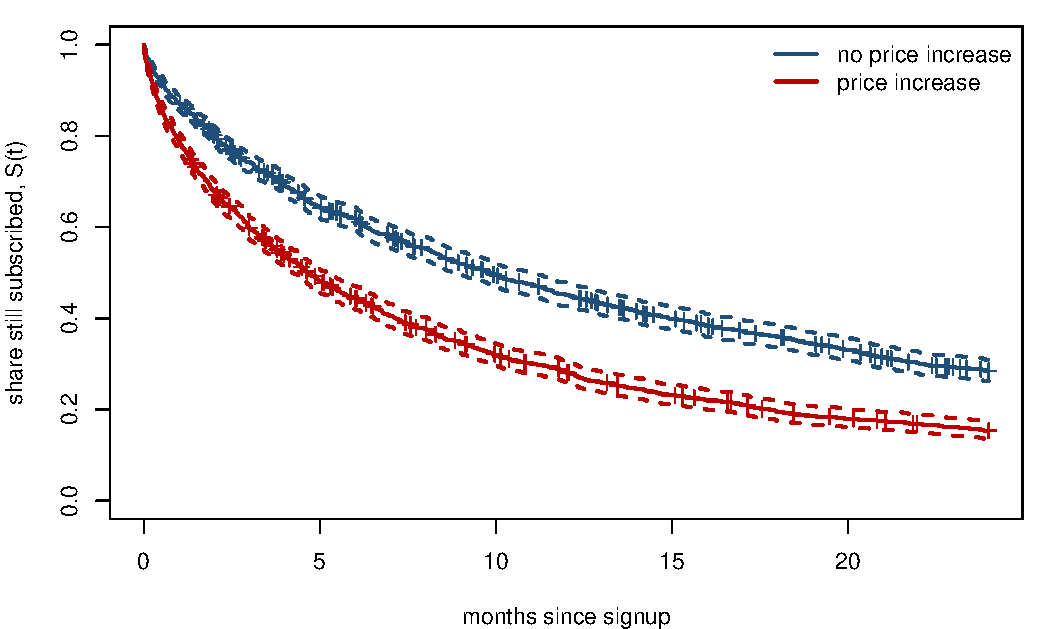
\includegraphics[width=.62\textwidth]{fig_dur_km.pdf}
\end{center}
\vspace{-.3cm}
{\small Nonparametric survival by group, censored spells marked. At each exit time $t_j$,
$\hat S(t) = \prod_{t_j \le t}(1 - d_j / n_j)$: exits over the number \emph{at risk}. Censored subscribers stay in
the denominator until they leave the data and never enter the numerator.}
\end{frame}


\begin{frame}{The censored likelihood}
Each subscriber contributes one of two things, exactly as in the Tobit:
\begin{align*}
	\ell(\theta) = \sum_i \Big[\, d_i \ln f(t_i \mid x_i; \theta) + (1 - d_i) \ln S(t_i \mid x_i; \theta) \,\Big]
	= \sum_i \Big[\, d_i \ln h(t_i \mid x_i; \theta) - \Lambda(t_i \mid x_i; \theta) \,\Big] .
\end{align*}
\begin{itemize}
	\item Completed spells ($d_i = 1$): the \alert{density} at the observed duration.
	\item Censored spells ($d_i = 0$): the \alert{probability} of lasting at least this long, $S(c_i)$.
	\medskip
	\item Second form uses $f = h S$ and $S = e^{-\Lambda}$: every spell pays the cumulative hazard for
	the time it was observed; completed spells also pay $\ln h$ at the moment of exit.
	\medskip
	\item Requires censoring to be \alert{independent} of $T$ given $x$: the data ending on 12/31 is fine;
	customers leaving the panel \emph{because} they are about to churn is not (that is selection again).
	\medskip
	\item Everything from Week 12 applies: score, Hessian, sandwich standard errors, likelihood-ratio tests.
\end{itemize}
\end{frame}


\begin{frame}{Parametric hazards: exponential and Weibull}
Proportional hazards form: $h(t \mid x) = h_0(t)\,\exp(x'\beta)$, with a parametric baseline.
\begin{itemize}
	\item \alert{Exponential}: $h_0(t) = \lambda$. Then $\Lambda(t \mid x) = \lambda t\,e^{x'\beta}$,
	$\E[T \mid x] = e^{-x'\beta}/\lambda$. One parameter, no duration dependence.
	\medskip
	\item \alert{Weibull}: $h_0(t) = \lambda p\,t^{\,p-1}$. $p < 1$ falling, $p = 1$ exponential, $p > 1$ rising.
	\medskip
	\item Interpretation of $\beta_j$: $\partial \ln h / \partial x_j$. $e^{\beta_j}$ is the \alert{hazard ratio}:
	the multiplicative effect on the exit rate, constant over $t$ by assumption.
	\medskip
	\item Software often reports the \alert{accelerated failure time} (AFT) form instead,
	$\ln T = \alpha + x'\gamma + \text{error}$: covariates stretch or compress time. For the Weibull the
	two are the same model with $\beta = -\gamma\,p$, and \texttt{survreg} in R uses AFT. Check which one
	you are reading before you interpret a sign.
	\medskip
	\item Wrong baseline shape biases $\hat\beta$ too, because the shape and the covariates compete to
	explain when exits happen. Next table.
\end{itemize}
\end{frame}


\begin{frame}{Cox: leave the baseline alone}
\begin{itemize}
	\item Cox (1972): keep $h(t \mid x) = h_0(t)\,e^{x'\beta}$ but do not specify $h_0$ at all.
	\medskip
	\item At each exit time $t_j$, ask: of everyone still at risk, why was it subscriber $j$ who left?
	\begin{align*}
		\Pr(j \text{ exits at } t_j \mid \text{one exit among the risk set } R_j)
		= \frac{h_0(t_j)\,e^{x_j'\beta}}{\sum_{k \in R_j} h_0(t_j)\,e^{x_k'\beta}}
		= \frac{e^{x_j'\beta}}{\sum_{k \in R_j} e^{x_k'\beta}} .
	\end{align*}
	The baseline cancels. Multiply these over exit times: the \alert{partial likelihood}. Maximize it.
	\medskip
	\item Each term is a conditional logit (Week 12) over who in the risk set exits. Censored spells
	sit in risk sets and then drop out; they never contribute a numerator.
	\medskip
	\item You get $\hat\beta$ and hazard ratios without ever estimating $h_0$; $\hat h_0$ can be recovered
	afterwards (Breslow) if you need predicted survival.
	\medskip
	\item Cost: proportionality is now the only assumption, and it is testable (interact $x$ with $\ln t$,
	or plot $\ln(-\ln \hat S)$ by group; parallel lines mean proportional hazards).
\end{itemize}
\end{frame}


\begin{frame}{Estimates on the simulated subscribers}
\begin{center}
\scriptsize
\begin{tabular}{lccccc}\toprule
 & Cox PH & Weibull PH & Exponential PH & OLS $\ln T$, uncensored only & OLS $\ln T$, censored as exits \\ \midrule
Price increase (truth $\beta = 0.5$; HR $= 1.65$) & 0.483 & 0.485 & 0.570 & -0.409 & -0.569 \\
 & (0.042) & (0.042) & (0.042) & (0.072) & (0.061) \\
Usage (truth $\beta = -0.4$) & -0.384 & -0.385 & -0.457 & 0.213 & 0.389 \\
 & (0.023) & (0.023) & (0.023) & (0.038) & (0.032) \\
Shape $p$ (truth $= 0.7$) & --- & 0.70 & 1 (imposed) & --- & --- \\
Baseline hazard & unrestricted & Weibull & constant & (AFT, wrong sign) & (AFT, wrong sign) \\
\bottomrule\end{tabular}

\end{center}
\medskip
\begin{itemize}
	\item Cox and Weibull agree with the truth and with each other; the Weibull also recovers the shape.
	\item The exponential imposes $p = 1$ and gets the covariate effects wrong, not just the baseline.
	\item The two OLS columns are the regressions people run before they learn this: dropping censored
	spells selects on short durations; treating them as exits mislabels the longest spells. Both have the
	wrong sign convention as well (AFT: higher hazard means \emph{shorter} $\ln T$).
\end{itemize}
\end{frame}


\begin{frame}{Unobserved heterogeneity: the hazard that falls though nobody's does}
\begin{center}
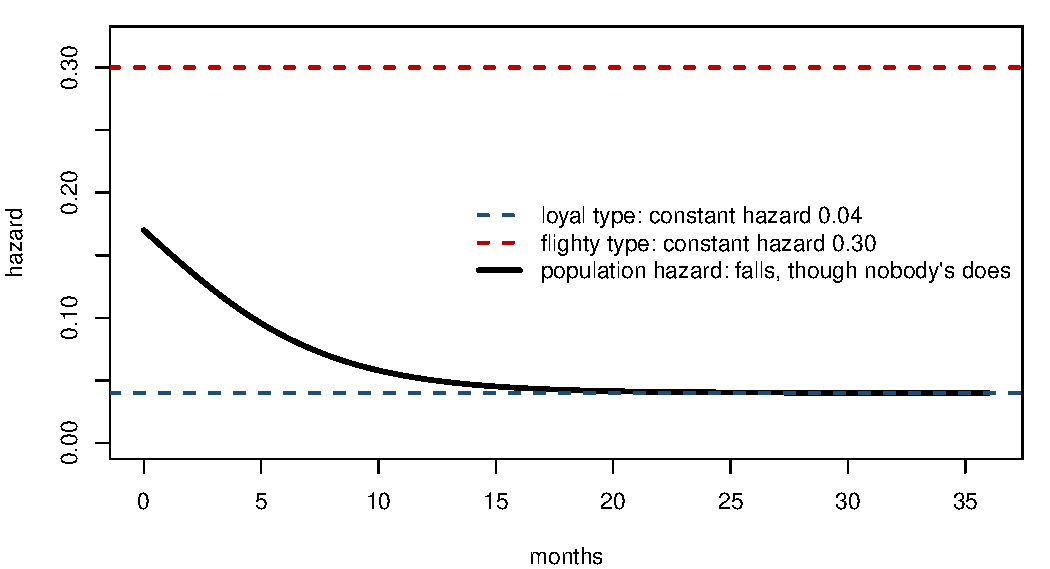
\includegraphics[width=.6\textwidth]{fig_dur_hetero.pdf}
\end{center}
\vspace{-.3cm}
\begin{itemize}
	\item Two types with \emph{constant} hazards. The flighty type leaves early; survivors are increasingly
	loyal. The population hazard falls: \alert{spurious negative duration dependence}.
	\item So a falling estimated hazard has two readings: individuals become less likely to leave over
	time, or the composition of who is left changes. Data on spells alone cannot tell them apart.
\end{itemize}
\end{frame}


\begin{frame}{What to do about heterogeneity}
\begin{itemize}
	\item \alert{Condition on more.} Covariates absorb some of the heterogeneity; the rest is a
	frailty term $\nu_i$ multiplying the hazard, $h(t \mid x, \nu) = \nu\,h_0(t)\,e^{x'\beta}$.
	\medskip
	\item \alert{Mixed proportional hazards.} Put a distribution on $\nu$ (gamma, usually) and
	integrate it out. Identified under proportionality with a covariate that shifts the hazard
	(Elbers--Ridder 1982), but fragile: $h_0$ and the distribution of $\nu$ are separated by functional form.
	\medskip
	\item \alert{Repeated spells} per unit (several subscriptions, several loans) identify $\nu_i$ from
	within-unit variation, the panel logic of Week 8. Much stronger.
	\medskip
	\item \alert{Even without a fix}, omitted $\nu$ biases $\hat\beta$ \emph{toward zero} as $t$ grows:
	high-$\nu$ units with hazard-raising $x$ leave first, so the estimated hazard ratio drifts even when
	the true one is constant.
	\medskip
	\item Treat estimated duration dependence as descriptive unless a design separates it from sorting.
\end{itemize}
\end{frame}


\begin{frame}{Design issues that come up every time}
\begin{itemize}
	\item \alert{Left truncation (delayed entry).} You start observing subscribers who signed up before
	your data began. They are in the data only because they survived to the start. Condition on
	$T > \text{entry time}$: risk sets must exclude units before they enter. Software handles it if you tell it.
	\medskip
	\item \alert{Time-varying covariates.} Price changes mid-spell. Split each spell into intervals with
	constant $x$ (``counting-process'' data); the likelihood in the second form on the earlier slide
	handles it directly. Cox handles it too.
	\medskip
	\item \alert{Competing risks.} A subscriber can cancel, or upgrade, or die. Treating the other exits
	as censoring gives the cause-specific hazard, which is fine for ``what raises cancellation?'' but
	not for ``what share will have cancelled by month 12?'' (that needs the cumulative incidence).
	\medskip
	\item \alert{Grouped time.} Monthly billing data records exits in months, not instants. Use the
	discrete-time model: a logit or complementary log-log on person-months with duration dummies.
	It is a panel logit, and it lets you use everything from Weeks 8 and 12.
\end{itemize}
\end{frame}


\begin{frame}[fragile]{In practice}
The \texttt{survival} package ships with R:
\begin{lstlisting}
library(survival)
km  <- survfit(Surv(time, event) ~ price, data = d);  plot(km)          # Kaplan-Meier
cox <- coxph(Surv(time, event) ~ price + usage, data = d)               # hazard ratios: exp(coef(cox))
wei <- survreg(Surv(time, event) ~ price + usage, data = d, dist = "weibull")
-coef(wei)[-1] / wei$scale;  1 / wei$scale                              # PH coefficients; shape p
\end{lstlisting}
Discrete time, with only \texttt{fixest}:
\begin{lstlisting}
pm <- expand_to_person_months(d)                                        # one row per subscriber-month at risk
feglm(exit ~ price + usage | month, data = pm, family = binomial("cloglog"))
\end{lstlisting}
\begin{itemize}
	\item The cloglog link makes the discrete-time model the exact grouped version of proportional
	hazards: coefficients are the same $\beta$. Month fixed effects are the baseline hazard.
	\item Python: \texttt{lifelines} (KM, Cox, Weibull) or the same person-month logit in \texttt{pyfixest}.
\end{itemize}
\end{frame}


\begin{frame}{Recap}
\begin{itemize}
	\item Model the \alert{hazard}: the exit rate given survival. It determines $S$, $f$, and $\E[T]$.
	\medskip
	\item Censored spells enter the likelihood through $S(c_i)$, completed ones through $f(t_i)$.
	Requires censoring independent of $T$ given $x$.
	\medskip
	\item Kaplan--Meier to look; Weibull or exponential when you want the shape; Cox when you do not
	want to assume it. Read AFT output carefully.
	\medskip
	\item A falling hazard is either duration dependence or sorting. Spell data alone cannot say which.
	\medskip
	\item Monthly data plus \texttt{fixest}: a person-month cloglog with month dummies \emph{is} a
	proportional-hazards model.
\end{itemize}
\end{frame}

\end{document}
